\subsection{Hardware test bed}
We conducted all benchmarks on a single CPU socket from Intel's \IVB and  \SKX families, respectively, since these  represent the oldest and the latest Intel architectures in active use within the scientific community at the time of writing:
\begin{itemize}
\item The \Intel \IVB architecture belongs to the class of ``classic'' designs with three inclusive cache levels. While the L1 and L2 caches are private to each core, the L3 cache is shared but scalabale in terms of bandwidth. The processor supports the AVX instruction set extension, which is capable of 256-bit wide \SIMD execution.
\item Contrary to its predecessors, the \Intel \SKX architecture has a shared but non-inclusive victim L3 cache and much larger private L2 caches. The model we use in this work supports AVX-512, which features 512-bit wide \SIMD execution.
%  \begin{comment}
%  \item {\GW \AMD \EPY is based on AMD's Zen microarchitecture. The basic building block of the architecture consists of Core Complex (CCX) consisting of three cores (can extend upto four on high end models) each having it's own private L1 and L2 cache. The L3 cache is shared between a core complex and is non-inclusive victim cache. A single socket of \EPY consists of eight such CCX.}
%  \end{comment}
 
\end{itemize}
Architectural details along with the attainable memory bandwidths are given in \cref{tab:test_bed}. 
All the measurements were done with \CPU clock speeds fixed at the indicated base frequencies. Note that for the \SKX architecture the clock frequency is scaled down internally to 2.2 \GHZ when using multi-core support and AVX-512 instruction set, however this is of minor importance for the algorithms discussed here.
\begin{comment}
\begin{table}[tbp]
\footnotesize
\caption{Compute node configurations. The last two columns present attainable bandwidth numbers ($b_S$) on a single socket, depending on the access pattern (copy vs. load only)}\label{tab:test_bed}
\begin{center}
%	\setlength{\tabcolsep}{3em}
	\begin{tabular}{|l| c  c c |}
		\toprule
		{Model name} & {Xeon\textsuperscript{\textregistered} E5-2660} & {Xeon\textsuperscript{\textregistered} Gold 6148} & { Epyc 7451 } \\
		\midrule
		{Microarchitecture} & {Ivy Bridge} & {Skylake} & {Zen} \\
		\midrule
		{Base clock frequency} & {2.2 GHz} & {2.4 GHz} & {2.3 GHz}\\
		{Physical Cores per socket} & {10} & {20} & {24}\\
		{L1d Cache} & {10 $\times$ 32 \KB} & {20 $\times$ 32 \KB} & {24 $\times$  32 \KB}\\
		{L2 Cache} & {10 $\times$ 256 \KB} & {20 $\times$ 1 \MB} & {24 $\times$ 512 \MB }\\
		{L3 Cache} & {25 \MB} & {27.5 \MB} & {8 $\times$ 8 \MB}\\
		{L3 type} & {inclusive} & {non-inclusive} & {non-inclusive}\\
		{Main Memory} & {32 GB} & {45 GB} & {4 $\times$ 16 GB}\\
		{Bandwidth per socket - load only} & {47 GB/s} & {115 GB/s} & {130 GB/s }\\ %TODO
		{Bandwidth per socket - copy} & {40 GB/s} & {104 GB/s} & {114 GB/s }\\
		\bottomrule
	\end{tabular}
\end{center}
\end{table} 
\end{comment}

\begin{table}[tbp]
	\footnotesize
	\caption{Technical details (per socket) about the Intel CPUs used for the benchmarks.}\label{tab:test_bed}
	\begin{center}
		%	\setlength{\tabcolsep}{3em}
		\begin{tabular}{l|cc}
			{Model name} & {Xeon\textsuperscript{\textregistered} E5-2660} & {Xeon\textsuperscript{\textregistered} Gold 6148} \\\midrule
			{Microarchitecture} & {\IVB} & {\SKX} \\\midrule
			{Base clock frequency} & {2.2 GHz} & {2.4 GHz}\\
			{Uncore clock frequency} & {2.2 GHz} & {2.4 GHz}\\
			{Physical cores per socket} & {10} & {20} \\
			{L1D cache} & {10 $\times$ 32 \KiB} & {20 $\times$ 32 \KiB}\\
			{L2 cache} & {10 $\times$ 256 \KiB} & {20 $\times$ 1 \MiB} \\
			{L3 cache} & {25 \MiB} & {27.5 \MiB}\\
			{L3 type} & {inclusive} & {non-inclusive, victim}\\
			{Main memory} & {32 \GiB} & {45 \GiB}\\
			{Bandwidth per socket, load-only} & {47 \GBS} & {115 \GBS}\\ %TODO
			{Bandwidth per socket, copy} & {40 \GBS} & {104 \GBS}\\
		\end{tabular}
	\end{center}
\end{table} 
As the attainable main memory bandwidth is the input parameter to the \roofline model used later, we have carefully measured this value depending on the data set size for two access patterns (copy and load-only). The data presented in \cref{fig:size_vs_bw} basically show the characteristic performance drop if data set size is too large to fit into the \acrfull{LLC}, which is L3 cache on both architectures (cf. \cref{tab:test_bed} for the actual sizes). 
\begin{figure}[tbp]
	\centering
	\subfloat[\emph{\IVB}]{\label{fig:ivy_size_vs_bw}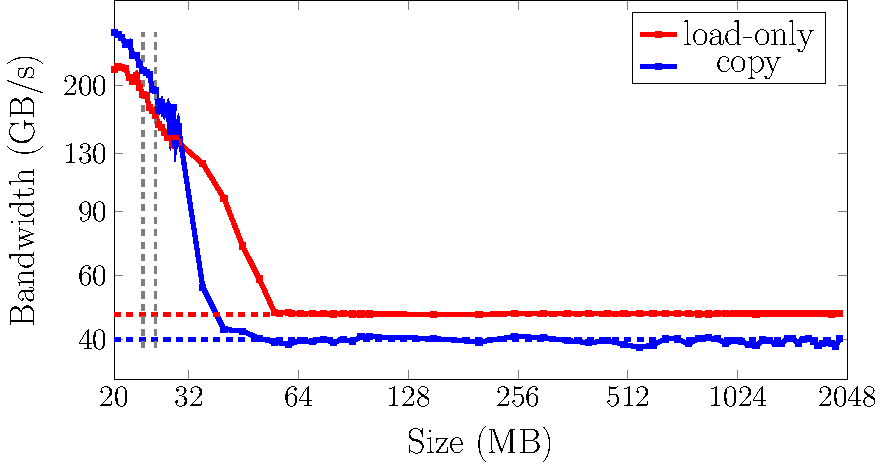
\includegraphics[width=0.5\textwidth , height=0.16\textheight]{pics/results/likwid_bench_bw/ivy}}
	\subfloat[\emph{\SKX}]{\label{fig:skx_size_vs_bw}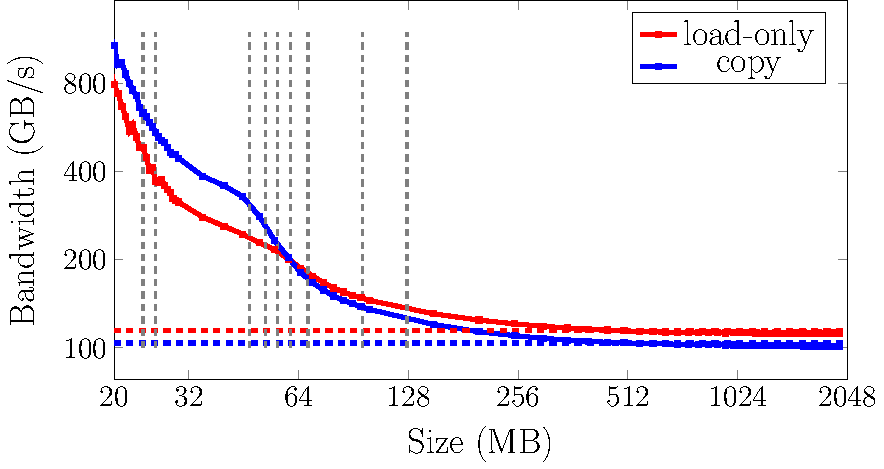
\includegraphics[width=0.5\textwidth , height=0.16\textheight]{pics/results/likwid_bench_bw/skx}}
	\caption{Attained bandwidth vs. total data size for range from 20 \MB to 2 \GB. The dotted lines show the asymptotic bandwidth given in \cref{tab:test_bed} for the load-only and copy benchmark. The benchmarks were performed on the full socket using the \likwidBench tool. Note, the logarithmic scales. The gray vertical lines correspond to the positions of matrices that might show caching effects, see \cref{subsec:bench_mat}.}
	\label{fig:size_vs_bw}
\end{figure}
Interestingly there is no sharp drop at the exact size of the \acrshort{LLC} but a rather steady performance decrease with enhanced data access rates also for data set sizes up to twice the \acrshort{LLC} size on \IVB. For \SKX this effect is even more pronounced as the non-inclusive victim L3 cache architecture only stores data which are not in L2 cache, thus the available cache size for an application may be the aggregate sizes of the L2 and L3 caches on this architecture.  The final bandwidth for the  \roofline model is chosen as the asymptotic value depicted in \cref{fig:size_vs_bw}. Of course caching effects are extremely sensitive to the data access pattern and thus the values presented here only provide simple upper bounds for the \acrshort{SymmSpMV} kernel with its potentially strong irregular data access. 

\subsection{External Tools and Software}
The following external libraries are used in this paper:
\begin{description}
	%TODO
	\item[\LIKWID 4.3.2] \cite{LIKWID}  \likwidPerfctr was used for counting hardware events and measuring derived metrics. The bandwidths shown in \cref{tab:test_bed} were taken by the  \likwidBench tool.
	\item[\COLPACK] \cite{COLPACK} was used for pre-processing matrices via \acrshort{MC}.
	\item[\SPMP] \cite{SpMP} was used to perform \acrshort{RCM}.
	\item[\METIS 5.1.0] \cite{METIS} was used for graph partitioning in \acrshort{ABMC}.
	\item[\acrshort{MKL} 19.0.2] \cite{MKL} was used for performing some reference sparse matrix computations.
\end{description}
All code was compiled with the Intel compiler in version 19.0.2 and the following compiler flags: {\tt -fno-alias -xHost -O3} for \IVB and {\tt -fno-alias -xCORE-AVX512 -O3} for \SKX.

\subsection{Benchmark Matrices}
\label{subsec:bench_mat}
Most test matrices were taken from the Suite\-Sparse Matrix Collection (former University of Florida Sparse Matrix Collection)~\cite{UOF} combining sets from two related papers \cite{RSB,park_ls}, which allows the reader to make straightforward comparison of results.  We also added some matrices from quantum physics applications, which originate from the particular project context in which RACE was developed~\cite{ESSEX}. All the matrices considered are real, although our underlying software would also support complex matrices.
%The selection of the matrices from SuiteSparse Matrix Collection is  mainly done by  Matrices from \ESSEX project are some of the matrices that are of interest in the iterative FEAST eigen value solver that internally uses Kaczmarz solver.
As mentioned before we restrict ourselves to matrices representing undirected graphs.
\cref{table:bench_matrices} gives an overview of the most important matrix properties like \acrfull{nrows}, \acrfull{nnz}, \acrfull{NNZR} along with the bandwidth of the matrix without ($bw$) and with ($bw_{RCM}$) \acrshort{RCM} pre-processing. 

Due to the extended cache size as seen in \cref{fig:size_vs_bw} it might happen that some of the matrices might attain higher effective bandwidths due to partial/full caching. The ten potential candidates for \SKX chip in terms of symmetric and full storage ($< 128 \MB$)  are marked with an asterisk in \cref{table:bench_matrices}, while only two among (\texttt{offshore} and \texttt{parabolic\_fem}) these satisfy the criteria for \IVB ($< 40 \MB$). The corresponding data set size for storing upper triangular part of these matrices have been labeled in \cref{fig:size_vs_bw}.

\begin{table}[tb]
	\footnotesize
	\caption{Details of the benchmark matrices. \acrshort{nrows} is the number of matrix rows and \acrshort{nnz} is the number of nonzeros. $\acrshort{NNZR}=\acrshort{nnz}/\acrshort{nrows}$ is the average number of nonzeros per row. $bw$ and $bw_{RCM}$ refers to the matrix bandwidth without and with \acrshort{RCM} pre-processing. Letter `C' in the parentheses of matrix name indicates a corner case matrix that will be discussed in detail, while letter `Q' marks a matrix from quantum physics that is not part of the SuiteSparse Matrix Collection. In asterisk (*) we have labeled all the matrices which are less than 128 \MB, which could potentially lead to some caching effects especially on \SKX architecture.} \label{tab:test_mtx}
	\label{table:bench_matrices}
	\begin{center}
		\begin{tabular}{|l|l|S[round-mode=places,round-precision=4]|S[round-mode=places,round-precision=4]|S[round-mode=places,round-precision=4]|S[round-mode=places,round-precision=4]|}
\toprule
\multirow{2}{*}{Index} & \multirow{2}{*}{Matrix name} & \multicolumn{3}{c|}{$\alpha_{SpMV}$} & {$I_{\acrshort{SpMV}}(\alpha_{SpMV})$} \\
%\midrule
\cline{3-6}
& &  {optimal} & {SKX} & {IVB} & {optimal}  \\
\midrule
{1}& {	crankseg\_1                }	& 0.004974840341951422	& 0.009900427637091272*	& 0.017876	& 0.16475420629866486	\\
{2}& {	ship\_003                  }	& 0.015054104375856307	& 0.029661678743938248*	& 0.039038	& 0.16101095659221026	\\
{3}& {	pwtk                      }	& 0.018730450092715727	& 0.03677214142565592*	& 0.038276	& 0.1596876177714501	\\
{4}& {	offshore                  }	& 0.061232390023872055	& 0.11539864519682566*	& 0.105831	& 0.14583098113326293	\\
{5}& {	F1                        }	& 0.012810282496064584	& 0.025296509558520128*	& 0.043622	& 0.16182947693011468	\\
{6}& {	inline\_1                  }	& 0.013681750417974054	& 0.013709	& 0.034046	& 0.16151058900649082	\\
{7}& {	parabolic\_fem             }	& 0.14309623622555628	& 0.25036603514337963*	& 0.224973	& 0.12494772020022805	\\
{8}& {	gsm\_106857                }	& 0.02708985058701268	& 0.052750692788036055*	& 0.094584	& 0.15675804527541276	\\
{9}& {	Fault\_639                 }	& 0.022324366119157866	& 0.045281	& 0.086085	& 0.15841480951843234	\\
{10}& {	Hubbard-12                }	& 0.07692947982285911	& 0.14286818452683273*	& 0.231786	& 0.14130255800224512	\\
{11}& {	Emilia\_923                }	& 0.022512653462004855	& 0.08265	& 0.085462	& 0.15834868547473438	\\
{12}& {	audikw\_1                  }	& 0.012152898336217176	& 0.062422	& 0.063762	& 0.16207086168751325	\\
{13}& {	bone010                   }	& 0.013768014517655372	& 0.049208	& 0.052338	& 0.16147909155409917	\\
{14}& {	dielFilterV3real          }	& 0.01234882033880347	& 0.072827	& 0.067509	& 0.16199884583462107	\\
{15}& {	thermal2                  }	& 0.14312355713563962	& 0.2504078517886007*	& 0.227709	& 0.12494174903463444	\\
{16}& {	Serena                    }	& 0.02156070528689192	& 0.100582	& 0.115621	& 0.15868356434880437	\\
{17}& {	Geo\_1438                  }	& 0.022768134283905977	& 0.089589	& 0.091725	& 0.15825905217944752	\\
{18}& {	Hook\_1498                 }	& 0.024591034497360605	& 0.103075	& 0.094818	& 0.1576224362116434	\\
{19}& {	Flan\_1565                 }	& 0.013328053114104274	& 0.054135	& 0.052516	& 0.161639862432339	\\
{20}& {	G3\_circuit                }	& 0.20695912474502637	& 0.34294305499160477*	& 0.335974	& 0.11239203379889182	\\
{21}& {	Anderson-16.5             }	& 0.14285714285714285	& 0.363368	& 0.318715	& 0.125	\\
{22}& {	FreeBosonChain-18         }	& 0.08024691655235494	& 0.27076	& 0.262774	& 0.14038128167567254	\\
{23}& {	nlpkkt120                 }	& 0.03657773850304069	& 0.160002	& 0.165642	& 0.15356057042478993	\\
{24}& {	channel-500x100x100-b050  }	& 0.05325806761196896	& 0.173504	& 0.133898	& 0.14824449726378677	\\
{25}& {	HPCG-192                  }	& 0.03742553488106633	& 0.135801	& 0.139089	& 0.15328119500901655	\\
{26}& {	FreeFermionChain-26       }	& 0.07396449704142012	& 0.387859	& 0.397282	& 0.1421362489486964	\\
{27}& {	Spin-26                   }	& 0.07142857142857142	& 0.367034	& 0.351781	& 0.14285714285714285	\\
{28}& {	Hubbard-14                }	& 0.06666796002509115	& 0.357508	& 0.359807	& 0.14423039256024434	\\
{29}& {	nlpkkt200                 }	& 0.036231752783504406	& 0.16692	& 0.172028	& 0.15367487636455557	\\
{30}& {	delaunay\_n24              }	& 0.1666668333335	& 0.406459	& 0.319197	& 0.1199999663999758	\\
{31}& {	Graphene-4096             }	& 0.0769548711240621	& 0.160392	& 0.127774	& 0.14129546073388705	\\
%#TABLE_DATA#
\bottomrule
\end{tabular}



	\end{center}
\end{table}

%\begin{table}[ht]
%	\footnotesize
%	\caption{Scamac matrices} \label{tab:test_mtx_scamac}
%	\begin{center}
%		\begin{tabular}{|l|l|S[round-mode=places,round-precision=4]|S[round-mode=places,round-precision=4]|S[round-mode=places,round-precision=4]|S[round-mode=places,round-precision=4]|}
\toprule
\multirow{2}{*}{Index} & \multirow{2}{*}{Matrix name} & \multicolumn{3}{c|}{$\alpha_{SpMV}$} & {$I_{\acrshort{SpMV}}(\alpha_{SpMV})$} \\
%\midrule
\cline{3-6}
& &  {optimal} & {SKX} & {IVB} & {optimal}  \\
\midrule
{1}& {	crankseg\_1                }	& 0.004974840341951422	& 0.009900427637091272*	& 0.017876	& 0.16475420629866486	\\
{2}& {	ship\_003                  }	& 0.015054104375856307	& 0.029661678743938248*	& 0.039038	& 0.16101095659221026	\\
{3}& {	pwtk                      }	& 0.018730450092715727	& 0.03677214142565592*	& 0.038276	& 0.1596876177714501	\\
{4}& {	offshore                  }	& 0.061232390023872055	& 0.11539864519682566*	& 0.105831	& 0.14583098113326293	\\
{5}& {	F1                        }	& 0.012810282496064584	& 0.025296509558520128*	& 0.043622	& 0.16182947693011468	\\
{6}& {	inline\_1                  }	& 0.013681750417974054	& 0.013709	& 0.034046	& 0.16151058900649082	\\
{7}& {	parabolic\_fem             }	& 0.14309623622555628	& 0.25036603514337963*	& 0.224973	& 0.12494772020022805	\\
{8}& {	gsm\_106857                }	& 0.02708985058701268	& 0.052750692788036055*	& 0.094584	& 0.15675804527541276	\\
{9}& {	Fault\_639                 }	& 0.022324366119157866	& 0.045281	& 0.086085	& 0.15841480951843234	\\
{10}& {	Hubbard-12                }	& 0.07692947982285911	& 0.14286818452683273*	& 0.231786	& 0.14130255800224512	\\
{11}& {	Emilia\_923                }	& 0.022512653462004855	& 0.08265	& 0.085462	& 0.15834868547473438	\\
{12}& {	audikw\_1                  }	& 0.012152898336217176	& 0.062422	& 0.063762	& 0.16207086168751325	\\
{13}& {	bone010                   }	& 0.013768014517655372	& 0.049208	& 0.052338	& 0.16147909155409917	\\
{14}& {	dielFilterV3real          }	& 0.01234882033880347	& 0.072827	& 0.067509	& 0.16199884583462107	\\
{15}& {	thermal2                  }	& 0.14312355713563962	& 0.2504078517886007*	& 0.227709	& 0.12494174903463444	\\
{16}& {	Serena                    }	& 0.02156070528689192	& 0.100582	& 0.115621	& 0.15868356434880437	\\
{17}& {	Geo\_1438                  }	& 0.022768134283905977	& 0.089589	& 0.091725	& 0.15825905217944752	\\
{18}& {	Hook\_1498                 }	& 0.024591034497360605	& 0.103075	& 0.094818	& 0.1576224362116434	\\
{19}& {	Flan\_1565                 }	& 0.013328053114104274	& 0.054135	& 0.052516	& 0.161639862432339	\\
{20}& {	G3\_circuit                }	& 0.20695912474502637	& 0.34294305499160477*	& 0.335974	& 0.11239203379889182	\\
{21}& {	Anderson-16.5             }	& 0.14285714285714285	& 0.363368	& 0.318715	& 0.125	\\
{22}& {	FreeBosonChain-18         }	& 0.08024691655235494	& 0.27076	& 0.262774	& 0.14038128167567254	\\
{23}& {	nlpkkt120                 }	& 0.03657773850304069	& 0.160002	& 0.165642	& 0.15356057042478993	\\
{24}& {	channel-500x100x100-b050  }	& 0.05325806761196896	& 0.173504	& 0.133898	& 0.14824449726378677	\\
{25}& {	HPCG-192                  }	& 0.03742553488106633	& 0.135801	& 0.139089	& 0.15328119500901655	\\
{26}& {	FreeFermionChain-26       }	& 0.07396449704142012	& 0.387859	& 0.397282	& 0.1421362489486964	\\
{27}& {	Spin-26                   }	& 0.07142857142857142	& 0.367034	& 0.351781	& 0.14285714285714285	\\
{28}& {	Hubbard-14                }	& 0.06666796002509115	& 0.357508	& 0.359807	& 0.14423039256024434	\\
{29}& {	nlpkkt200                 }	& 0.036231752783504406	& 0.16692	& 0.172028	& 0.15367487636455557	\\
{30}& {	delaunay\_n24              }	& 0.1666668333335	& 0.406459	& 0.319197	& 0.1199999663999758	\\
{31}& {	Graphene-4096             }	& 0.0769548711240621	& 0.160392	& 0.127774	& 0.14129546073388705	\\
%#TABLE_DATA#
\bottomrule
\end{tabular}



%	\end{center}
%\end{table}

%\begin{table}[ht]
%	\footnotesize
%	\caption{nlpkkt matrices} \label{tab:test_mtx_nlpkkt}
%	\begin{center}
%		\begin{tabular}{|l|l|S[round-mode=places,round-precision=4]|S[round-mode=places,round-precision=4]|S[round-mode=places,round-precision=4]|S[round-mode=places,round-precision=4]|}
\toprule
\multirow{2}{*}{Index} & \multirow{2}{*}{Matrix name} & \multicolumn{3}{c|}{$\alpha_{SpMV}$} & {$I_{\acrshort{SpMV}}(\alpha_{SpMV})$} \\
%\midrule
\cline{3-6}
& &  {optimal} & {SKX} & {IVB} & {optimal}  \\
\midrule
{1}& {	crankseg\_1                }	& 0.004974840341951422	& 0.009900427637091272*	& 0.017876	& 0.16475420629866486	\\
{2}& {	ship\_003                  }	& 0.015054104375856307	& 0.029661678743938248*	& 0.039038	& 0.16101095659221026	\\
{3}& {	pwtk                      }	& 0.018730450092715727	& 0.03677214142565592*	& 0.038276	& 0.1596876177714501	\\
{4}& {	offshore                  }	& 0.061232390023872055	& 0.11539864519682566*	& 0.105831	& 0.14583098113326293	\\
{5}& {	F1                        }	& 0.012810282496064584	& 0.025296509558520128*	& 0.043622	& 0.16182947693011468	\\
{6}& {	inline\_1                  }	& 0.013681750417974054	& 0.013709	& 0.034046	& 0.16151058900649082	\\
{7}& {	parabolic\_fem             }	& 0.14309623622555628	& 0.25036603514337963*	& 0.224973	& 0.12494772020022805	\\
{8}& {	gsm\_106857                }	& 0.02708985058701268	& 0.052750692788036055*	& 0.094584	& 0.15675804527541276	\\
{9}& {	Fault\_639                 }	& 0.022324366119157866	& 0.045281	& 0.086085	& 0.15841480951843234	\\
{10}& {	Hubbard-12                }	& 0.07692947982285911	& 0.14286818452683273*	& 0.231786	& 0.14130255800224512	\\
{11}& {	Emilia\_923                }	& 0.022512653462004855	& 0.08265	& 0.085462	& 0.15834868547473438	\\
{12}& {	audikw\_1                  }	& 0.012152898336217176	& 0.062422	& 0.063762	& 0.16207086168751325	\\
{13}& {	bone010                   }	& 0.013768014517655372	& 0.049208	& 0.052338	& 0.16147909155409917	\\
{14}& {	dielFilterV3real          }	& 0.01234882033880347	& 0.072827	& 0.067509	& 0.16199884583462107	\\
{15}& {	thermal2                  }	& 0.14312355713563962	& 0.2504078517886007*	& 0.227709	& 0.12494174903463444	\\
{16}& {	Serena                    }	& 0.02156070528689192	& 0.100582	& 0.115621	& 0.15868356434880437	\\
{17}& {	Geo\_1438                  }	& 0.022768134283905977	& 0.089589	& 0.091725	& 0.15825905217944752	\\
{18}& {	Hook\_1498                 }	& 0.024591034497360605	& 0.103075	& 0.094818	& 0.1576224362116434	\\
{19}& {	Flan\_1565                 }	& 0.013328053114104274	& 0.054135	& 0.052516	& 0.161639862432339	\\
{20}& {	G3\_circuit                }	& 0.20695912474502637	& 0.34294305499160477*	& 0.335974	& 0.11239203379889182	\\
{21}& {	Anderson-16.5             }	& 0.14285714285714285	& 0.363368	& 0.318715	& 0.125	\\
{22}& {	FreeBosonChain-18         }	& 0.08024691655235494	& 0.27076	& 0.262774	& 0.14038128167567254	\\
{23}& {	nlpkkt120                 }	& 0.03657773850304069	& 0.160002	& 0.165642	& 0.15356057042478993	\\
{24}& {	channel-500x100x100-b050  }	& 0.05325806761196896	& 0.173504	& 0.133898	& 0.14824449726378677	\\
{25}& {	HPCG-192                  }	& 0.03742553488106633	& 0.135801	& 0.139089	& 0.15328119500901655	\\
{26}& {	FreeFermionChain-26       }	& 0.07396449704142012	& 0.387859	& 0.397282	& 0.1421362489486964	\\
{27}& {	Spin-26                   }	& 0.07142857142857142	& 0.367034	& 0.351781	& 0.14285714285714285	\\
{28}& {	Hubbard-14                }	& 0.06666796002509115	& 0.357508	& 0.359807	& 0.14423039256024434	\\
{29}& {	nlpkkt200                 }	& 0.036231752783504406	& 0.16692	& 0.172028	& 0.15367487636455557	\\
{30}& {	delaunay\_n24              }	& 0.1666668333335	& 0.406459	& 0.319197	& 0.1199999663999758	\\
{31}& {	Graphene-4096             }	& 0.0769548711240621	& 0.160392	& 0.127774	& 0.14129546073388705	\\
%#TABLE_DATA#
\bottomrule
\end{tabular}



%	\end{center}
%\end{table}

\subsection{Kernels} \label{subsec:test_kernels}
We evaluate our methods by parallelization of the \acrfull{SymmSpMV} kernel using \DTWO coloring, which avoids concurrent update of the same vector entries by different threads. 

%In this case, the result is identical to the serial code (``exact kernel''). As an example of an iterative solver we have chosen \acrfull{SymmKACZ}. It reads and writes indirectly from the same vector, which leads to a change in convergence depending on the coloring scheme (``inexact kernel'').
% {\GW To be done As an example for an iterative solver with distance2 dependency we have chosen the \acrshort{KACZ} ...}

Since the kernel is closely related to the \acrshort{SpMV} kernel by structure and computational intensity, we start with a discussion of \acrshort{SpMV} and extend it towards \acrshort{SymmSpMV} later. In all cases the aim is to derive realistic upper performance bounds, which can be estimated once the computational intensity and main memory bandwidth (\acrshort{b_s}, see \cref{tab:test_bed}) is known \cite{Williams_roofline}, \ie
  \begin{align}
   	\label{eq:upper_performance}
   	P_\mathrm{kernel}  &= I_\mathrm{kernel}  \times b_S
  \end{align}
%Our kernels have considerably more loads compared to stores, therefore we choose $b_s$ to be the most optimistic (load-only) value from \cref{tab:test_bed}.
Since bandwidth ($b_s$) depends on the ratio of load to store streams we present the model for both upper (load-only) and lower bound (copy) bandwidth case.  
 % Due to the nature of our kernels and matrices having considerable amount of nonzeros our algorithms have considerably more loads compared to stores, therefore we choose $b_s$ to be the most optimistic (load-only) value from \cref{tab:test_bed} if not mentioned otherwise.
  
  In the following we choose the \acrshort{CRS} storage format for the  implementation of \acrshort{SpMV} as well as  \acrshort{SymmSpMV} and assume symmetric matrices.

\subsubsection{\acrshort{SpMV}}
A baseline \acrshort{SpMV} kernel is presented in \Cref{alg:SpMV}. It has no loop-carried dependencies, so parallelization of the outer loop using, \eg OpenMP, is straightforward. 
\begin{algorithm}[tbp]
	\caption{Sparse matrix-vector multiplication (\acrshort{SpMV}) using the compressed sparse row (\acrshort{CRS}) format: $b=A x$} 
	\label{alg:SpMV}
	\begin{algorithmic}[1]
	    \STATE{$double:: A[nnz], b[nrows], x[nrows]$}
	    \STATE{$integer:: col[nnz], rowPtr[nrows+1], tmp$}
		\FOR{$row=1:nrows$}
			\STATE{$tmp=0$}
			\FOR{$idx=rowPtr[row]:rowPtr[row+1]$}
				\STATE{$tmp += A[idx]*x[col[idx]]$} 
			\ENDFOR
			\STATE{$b[row] = tmp$}
		\ENDFOR
	\end{algorithmic}
\end{algorithm}
Following the discussion in~\cite{Moritz_sell}, its computational intensity is
\begin{equation}
\label{eq:SpMV_intensity}
I_\mathrm{\acrshort{SpMV}} (\alpha)= \frac{2}{8+4+8\alpha+\frac{20}{\acrshort{NNZR}}} \frac{\FLOP}{\BYTE}\eos
\end{equation}
Here we assume that the matrix data  ($A[], col[]$), the LHS vector ($b[]$) and the row pointer information ($rowPtr[]$) are loaded only once from main memory, since these data structures are consecutively accessed. The intensity is calculated from the average cost of performing all computations required for one nonzero element of the matrix. Thus, contributions which are independent of the inner (short) loop are rescaled by $\acrshort{NNZR}$, which is the average number of nonzeros per row (i.e., the average length of the inner loop). 

The $8\alpha$ term quantifies the data traffic caused by accessing the right hand side (RHS) vector ($x[]$). The value of $\alpha$ depends on the matrix structure as well as on the RHS vector data set size and the available cache size. The minimum value of $\alpha=\acrshort{NNZR}^{-1}$ is attained if the RHS vector is only loaded once from main memory to the cache and all subsequent accesses in the same \acrshort{SpMV} are cache hits. This limit is typically observed for matrices with low bandwidth (high access locality) or if the cache is large enough to hold the full RHS data during one \acrshort{SpMV}. The actual value of $\alpha$ can be determined experimentally by measuring the data traffic when executing the \acrshort{SpMV}; see~\cite{Moritz_sell} for more details.\footnote{In~\cite{Moritz_sell} the traffic for the row pointer was not accounted for, \ie the denominator in (\ref{eq:SpMV_intensity}) is larger by $\frac{4}{\acrshort{NNZR}}\,\BYTE$. This error is only significant when $\acrshort{NNZR}$ is small.}  The optimal value of $\alpha$ ($\acrshort{NNZR}^{-1}$) together with the corresponding intensity value as well as the measured $\alpha$ values (denoted by $\alpha_\mathrm{\acrshort{SpMV}}$) for all matrices on the two processor chips are given in \cref{table:alpha_values}. 
\begin{table}[htbp]
	\footnotesize
	\caption{The optimal value and the measured values of $\alpha_{\acrshort{SpMV}}$ on \SKX (SKX) as well as \IVB (IVB) for the \acrshort{SpMV} kernel (using the \LIKWID tool) are presented in columns three to five. Following \cref{eq:upper_performance} the maximum \acrshort{SpMV} performance can be calculated for each architecture using the best intensity values  ($I_{\acrshort{SpMV}}(\alpha_{SpMV})$ in $\frac{\FLOP}{\BYTE}$) as shown in the last column.}
	\label{table:alpha_values}
	\begin{center}
		\begin{tabular}{|l|l|S[round-mode=places,round-precision=4]|S[round-mode=places,round-precision=4]|S[round-mode=places,round-precision=4]|S[round-mode=places,round-precision=4]|}
\toprule
\multirow{2}{*}{Index} & \multirow{2}{*}{Matrix name} & \multicolumn{3}{c|}{$\alpha_{SpMV}$} & {$I_{\acrshort{SpMV}}(\alpha_{SpMV})$} \\
%\midrule
\cline{3-6}
& &  {optimal} & {SKX} & {IVB} & {optimal}  \\
\midrule
{1}& {	crankseg\_1                }	& 0.004974840341951422	& 0.009900427637091272*	& 0.017876	& 0.16475420629866486	\\
{2}& {	ship\_003                  }	& 0.015054104375856307	& 0.029661678743938248*	& 0.039038	& 0.16101095659221026	\\
{3}& {	pwtk                      }	& 0.018730450092715727	& 0.03677214142565592*	& 0.038276	& 0.1596876177714501	\\
{4}& {	offshore                  }	& 0.061232390023872055	& 0.11539864519682566*	& 0.105831	& 0.14583098113326293	\\
{5}& {	F1                        }	& 0.012810282496064584	& 0.025296509558520128*	& 0.043622	& 0.16182947693011468	\\
{6}& {	inline\_1                  }	& 0.013681750417974054	& 0.013709	& 0.034046	& 0.16151058900649082	\\
{7}& {	parabolic\_fem             }	& 0.14309623622555628	& 0.25036603514337963*	& 0.224973	& 0.12494772020022805	\\
{8}& {	gsm\_106857                }	& 0.02708985058701268	& 0.052750692788036055*	& 0.094584	& 0.15675804527541276	\\
{9}& {	Fault\_639                 }	& 0.022324366119157866	& 0.045281	& 0.086085	& 0.15841480951843234	\\
{10}& {	Hubbard-12                }	& 0.07692947982285911	& 0.14286818452683273*	& 0.231786	& 0.14130255800224512	\\
{11}& {	Emilia\_923                }	& 0.022512653462004855	& 0.08265	& 0.085462	& 0.15834868547473438	\\
{12}& {	audikw\_1                  }	& 0.012152898336217176	& 0.062422	& 0.063762	& 0.16207086168751325	\\
{13}& {	bone010                   }	& 0.013768014517655372	& 0.049208	& 0.052338	& 0.16147909155409917	\\
{14}& {	dielFilterV3real          }	& 0.01234882033880347	& 0.072827	& 0.067509	& 0.16199884583462107	\\
{15}& {	thermal2                  }	& 0.14312355713563962	& 0.2504078517886007*	& 0.227709	& 0.12494174903463444	\\
{16}& {	Serena                    }	& 0.02156070528689192	& 0.100582	& 0.115621	& 0.15868356434880437	\\
{17}& {	Geo\_1438                  }	& 0.022768134283905977	& 0.089589	& 0.091725	& 0.15825905217944752	\\
{18}& {	Hook\_1498                 }	& 0.024591034497360605	& 0.103075	& 0.094818	& 0.1576224362116434	\\
{19}& {	Flan\_1565                 }	& 0.013328053114104274	& 0.054135	& 0.052516	& 0.161639862432339	\\
{20}& {	G3\_circuit                }	& 0.20695912474502637	& 0.34294305499160477*	& 0.335974	& 0.11239203379889182	\\
{21}& {	Anderson-16.5             }	& 0.14285714285714285	& 0.363368	& 0.318715	& 0.125	\\
{22}& {	FreeBosonChain-18         }	& 0.08024691655235494	& 0.27076	& 0.262774	& 0.14038128167567254	\\
{23}& {	nlpkkt120                 }	& 0.03657773850304069	& 0.160002	& 0.165642	& 0.15356057042478993	\\
{24}& {	channel-500x100x100-b050  }	& 0.05325806761196896	& 0.173504	& 0.133898	& 0.14824449726378677	\\
{25}& {	HPCG-192                  }	& 0.03742553488106633	& 0.135801	& 0.139089	& 0.15328119500901655	\\
{26}& {	FreeFermionChain-26       }	& 0.07396449704142012	& 0.387859	& 0.397282	& 0.1421362489486964	\\
{27}& {	Spin-26                   }	& 0.07142857142857142	& 0.367034	& 0.351781	& 0.14285714285714285	\\
{28}& {	Hubbard-14                }	& 0.06666796002509115	& 0.357508	& 0.359807	& 0.14423039256024434	\\
{29}& {	nlpkkt200                 }	& 0.036231752783504406	& 0.16692	& 0.172028	& 0.15367487636455557	\\
{30}& {	delaunay\_n24              }	& 0.1666668333335	& 0.406459	& 0.319197	& 0.1199999663999758	\\
{31}& {	Graphene-4096             }	& 0.0769548711240621	& 0.160392	& 0.127774	& 0.14129546073388705	\\
%#TABLE_DATA#
\bottomrule
\end{tabular}



	\end{center}
\end{table}
 Choosing the matrices 10, 22 and 31, which have approximately the same optimal $\alpha_{\acrshort{SpMV}}$, one can study the delicate influence of matrix structure (i.e. matrix bandwidth and number of rows; see \cref{tab:test_mtx}) and the cache size on the actual data traffic, i.e. the measured values of $\alpha_{\acrshort{SpMV}}$.
 
For most of the ten candidate matrices on \SKX architecture that could potentially show caching effect (see \cref{table:bench_matrices}) we observe the measured $\alpha_{\acrshort{SpMV}}$ to be lower than optimal. In this case we set their values to the optimal alpha value of \acrshort{SymmSpMV} ($\alpha_{\acrshort{SymmSpMV}}$) which will be defined in the following \cref{sect:SymmSpmv}. These cases are marked with asterisk in \cref{table:alpha_values}.
 
\begin{comment}
\subsubsection{\SpMTV}
Sparse Matrix Transpose Vector multiplication (\SpMTV) is a kernel with a \DTWO dependency.
\begin{algorithm}[H]
	\caption{SpMTV Find $b$ : $b=A'x$} 
	\label{alg:SpMTV}
	\begin{algorithmic}[1]
		\FOR{$row=1:nrows$}
		\FOR{$idx=rowPtr[row]:rowPtr[row+1]$}
		\STATE{$b[col[idx]] += A[idx]*x[row]$} 
		\ENDFOR
		\ENDFOR
	\end{algorithmic}
\end{algorithm}
In comparison to \acrshort{SpMV} it requires scattered writes, which require attention in order to avoid race conditions when executing in parallel. The arithmetic intensity of the kernel $I_\mathrm{\SpMTV}$ is
\begin{equation}
\label{eq:SpMTV_intensity}
I_\mathrm{\SpMTV} (\alpha)= \frac{2}{8+4+16*\alpha+\frac{8}{\acrshort{NNZR}}} \\
\end{equation}
In ideal case data traffic for this kernel should remain close to that of SpMV, if \acrshort{NNZR} are sufficiently high, and $\alpha$ factor is small enough.
\end{comment}

\subsubsection{\acrshort{SymmSpMV}}
\label{sect:SymmSpmv}

\Acrshort{SymmSpMV} exploits the symmetry of the matrix ($A_{ij}=A_{ji}$) to reduce storage size for matrix data and reduce the overall memory traffic by operating on the upper (or lower) half of the matrix only. Thus for every nonzero matrix entry we need to update two entries in the LHS vector ($b[]$) as shown in~\cref{alg:SymmSpMV}.
\begin{algorithm}[tbp]
	\caption{SymmSpMV $b=Ax$, where $A$ is an upper triangular matrix} 
	\label{alg:SymmSpMV}
	\begin{algorithmic}[1]
		\FOR{$row=1:nrows$}
		\STATE{$diag\_idx=rowPtr[row]$}
		\STATE{$b[row] += A[diag\_idx]*x[row]$}
			\STATE{$tmp = 0$}
			\FOR{$idx=rowPtr[row]+1:rowPtr[row+1]$}
				\STATE{$tmp += A[idx]*x[col[idx]]$}
				\STATE{$b[col[idx]] += A[idx]*x[row]$} 
			\ENDFOR
			\STATE{$b[row] += tmp$}
		\ENDFOR
	\end{algorithmic}
\end{algorithm}
In line with the discussion above, the computational intensity of \acrshort{SymmSpMV} is
\begin{align}
\label{eq:SymmSpMV_intensity}
I_\mathrm{\acrshort{SymmSpMV}} (\alpha) &= \frac{4}{8+4+24*\alpha+\frac{4}{\acrshort{SymmNNZR}}} \frac{\FLOP}{\BYTE}\cma\\
\label{eq:NNZR_symm}
\text{ where  } \acrshort{SymmNNZR} &= (\acrshort{NNZR}-1)/2 + 1\eos
\end{align}

For a given nonzero matrix element, $4~\FLOP$, i.e., twice the amount of work than in \acrshort{SpMV} is performed. In addition we have indirect access to the LHS vector (read and write) which triples the traffic contribution quantified by $\alpha$\@. The only term scaled with \acrshort{SymmNNZR} (number of nonzeros per row in the upper triangular part of the matrix) is the row pointer. The most optimistic value of $\alpha$ ($\alpha_{\acrshort{SymmSpMV}}$) in this case is $1/{\acrshort{SymmNNZR}}$, which correspond to one time transfer of the LHS and RHS vector.  Note that the $\alpha$ for \acrshort{SpMV} and \acrshort{SymmSpMV} may be different even for the same matrix and the same compute device, as in the latter case the two vectors are accessed irregularly and compete for the same amount of cache. Thus we can assume that the $\alpha$ value measured for \acrshort{SpMV} ($\alpha_\mathrm{\acrshort{SpMV}}$) is a lower bound for \acrshort{SymmSpMV}. Since an upper bound for performance is the product of computational intensity and the main memory bandwidth (see \cref{eq:upper_performance}), this approach provides an upper performance bound for \acrshort{SymmSpMV}.  However, note that the performance models derived for matrices having caching effects (see \cref{table:alpha_values}) need not be strictly upper bound, as it heavily depends on  the caching strategy of the underlying architecture.
\begin{comment}
 for a given matrix structure:
 \begin{align}
\label{eq:SymmSpMV_performance}
P^{max}_\mathrm{\acrshort{SymmSpMV}}  &= I_\mathrm{\acrshort{SymmSpMV}} (\alpha_\mathrm{\acrshort{SpMV}})  \times b_S
\end{align}
As most matrices have a considerable number of nonzeros per row, we chose $b_S$ to be the optimistic (load-only) value  from~\cref{tab:test_bed}.
\end{comment}

Comparing~\cref{eq:SymmSpMV_intensity} and~\cref{eq:SpMV_intensity} it is obvious that the perfect speed-up of 2$\times$ when using \acrshort{SymmSpMV} instead of \acrshort{SpMV} is only attainable in the limit of small $\alpha$\@. %, \ie for regularly structured matrices or low-bandwidth matrices.
Considering the large prefactor of the $\alpha$ contribution, any implementation of \acrshort{SymmSpMV} must aim at ensuring high data locality. The indirect update of the LHS has also large impact on parallelization strategy as two rows which have a nonzero in the same column can not be computed in parallel. In a graph-based approach to this problem this is equivalent to the constraint that only vertices can be computed in parallel which have at least distance two.

\begin{comment}
\subsubsection{\GS and \SYMMGS}
Gauss-Seidel (\GS) is a solver having \DONE dependency. Contrary to the above kernels \GS is in-exact meaning it is an iterative method. \Cref{alg:GS} shows the Gauss-Seidel algorithm where its assumed that the diagonal entries of the matrix are stored as first entry in their corresponding rows.
\begin{algorithm}[H]
	\caption{GS Solve for $x$ : $Ax=b$} 
	\label{alg:GS}
	\begin{algorithmic}[1]
		\FOR{$row=1:nrows$}
		\STATE{$x[row]+=b[row]$}
		\FOR{$idx=rowPtr[row]+1:rowPtr[row+1]$}
		\STATE{$x[row] -= A[idx]*x[col[idx]]$} 
		\ENDFOR
		\STATE{$diag=A[rowPtr[row]]$}
		\STATE{$x[row]/=diag$}
		\ENDFOR
	\end{algorithmic}
\end{algorithm}
Regarding the in-core execution the kernel has same properties as of \acrshort{SpMV}, but requires an additional divide operation per row of the matrix. If the locality ($\alpha$ factor) is not disturbed due to pre-processing the kernel requires same data traffic as of \acrshort{SpMV}. The arithmetic intensity of \GS is the same as that of \acrshort{SpMV}, if we neglect the divide operation that occurs once per every row.
\begin{equation}
\label{eq:GS_intensity}
I_\mathrm{GS} = I_\mathrm{SPMV}
\end{equation}



In general for most of the algorithms one is interested in symmetric operator therefore commonly one would encounter symmetric variant of Gauss-Seidel, so called symmetric Gauss-Seidel (\SYMMGS). The algorithm remains same except that instead of just doing forward sweep shown in \cref{alg:GS} one would follow it with a backward sweep \ie {\tt row=nrows:-1:1}. The intensity of \SYMMGS remains same as of \GS, as we do two times more flops and bring in proportional data.
\end{comment}

\begin{comment}
\subsubsection{\acrshort{KACZ} and \acrshort{SymmKACZ}}
The iterative Kaczmarz solver is a row-projection algorithm with a data dependency.
%The update step for solving $x$ in $Ax = b$ is shown in \cref{eq:KACZ}.
A new approximation $x^{k+1}$ for solving $x$ in $Ax = b$ is obtained by projecting  the current iterate $x^{k}$ to the $i$-th linear equation $A_i$: 
\begin{equation}
	\label{eq:KACZ}
	x^{k+1} = x^{k} + \frac{b_i - \langle A_i, x_k \rangle}{\|A_i\|^2} \bar{A_i}\eos
\end{equation}
The basic compute kernel (\acrshort{KACZ}) is  presented in~\cref{alg:KACZ}. For its parallelization one typically uses a \DTWO coloring of the graph representing the matrix. As this does not lead to the same result as for the serial execution of the kernel, the actual coloring scheme may impact the convergence of the iterative scheme.

\begin{algorithm}[tbp]
	\caption{KACZ kernel used for solving $Ax=b$; outer iteration loop not shown} 
	\label{alg:KACZ}
	\begin{algorithmic}[1]
		\FOR{$row=1:nrows$}
		\STATE{$row\_norm=0$}
		\STATE{$scale=b[row]$}
		\FOR{$idx=rowPtr[row]:rowPtr[row+1]$}
		\STATE{$scale -= A[idx]*x[col[idx]]$}
		\STATE{$rownorm += A[idx]*A[idx]$} 
		\ENDFOR
		\STATE{$scale=scale/rownorm$}
		\FOR{$idx=rowPtr[row]:rowPtr[row+1]$}
		\STATE{$x[col[idx]] += scale*A[idx]$} 
		\ENDFOR
		\ENDFOR
	\end{algorithmic}
\end{algorithm}
From a computational perspective the kernel is closely related to \acrshort{SpMV} and \acrshort{SymmSpMV} but performs an in-place indirect vector update ($x[col[]]$). This vector update is the only contribution to $\alpha$, so the computational intensity is\footnote{The computation of $rownorm$ in each row can be avoided if the system  (matrix $A[]$ and vector $b[]$) is pre-scaled, which reduces the numerator from 6 to 4 \FLOP. Note, however, that the time to solution will remain the same, since this kernel is usually memory bound.}
\begin{equation}
\label{eq:KACZ_intensity}
I_\mathrm{KACZ} (\alpha) =  \frac{6}{8+4+16*\alpha+\frac{12}{\acrshort{NNZR}}} \frac{\FLOP}{\BYTE} \eos
\end{equation}
Having two short inner loops does not impact the overall memory traffic (and also the computational intensity) as the data can be kept in some inner cache  between the two inner loops. We can also ignore the impact of the divide operation as it is only done once per row and its cost is negligible for main memory bandwidth- or latency-bound scenarios.  

A variant of the algorithm called symmetric Kaczmarz (\acrshort{SymmKACZ}) uses a symmetric operator: The  forward sweep shown in \cref{alg:KACZ} is followed by a backward sweep, in which the outermost loop is traversed in reverse order.
%\ie { \tt row=nrows:-1:1} in~\cref{alg:KACZ}.
This does not change the computational intensity.

%Symmetric variant of \acrshort{KACZ} is denoted by \acrshort{SymmKACZ}, and similar to \SYMMGS this requires forward sweep followed by a backward sweep. 
\end{comment}